\documentclass{astroedu-lab}

\begin{document}

\pagestyle{plain}

\begin{problem}{\huge Радиотехническая работа 19\\\\Безынерционные линейные цепи\\\\Выполнил Жданов Елисей Б01-205}

\section{[Оборудование:]}

Макетная плата

Набор резисторов и конденсаторов различных номиналов

Электронный осциллограф на печатной плате

Электронный генератор сигналов на печатной плате

ПО MicroCap 10.0.8.0

\section{Задание}

\subsection{Звенья Саллена-Ки}

\begin{figure}[!h]
	\centering
	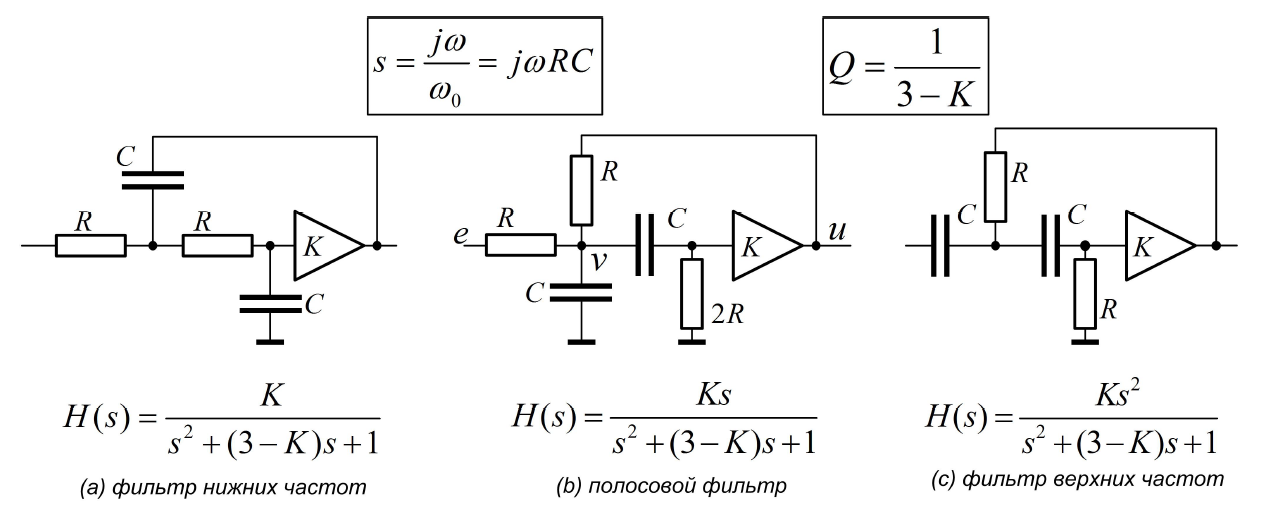
\includegraphics[width=0.9\textwidth]{sall.png}
	\label{fig:boiler}
\end{figure}

\subsubsection{Теория}

Звенья Саллена-Ки, рис. 10, используют неинвертирующий усилитель с коэффициентом усиления $K<3$. Они просты как схемотехнически, так и в плане расчета. Резонансная частот звена задается выбором постоянной времени $R C: \omega_0=1 / R C$, а добротность $Q=1 /(3-K)$ зависит только от усиления. Попытка достижения этими звеньями высоких значений добротности наталкивается на проблему точности задания коэффициента усиления. Скажем, чтобы получить добротность $Q=100$, нужно иметь $K=2.99$, и это при том, что при $K>3$ звено теряет устойчивость.

\subsubsection{Выполнение}

1) Откроем модель \textit{skey.cir} звеньев Саллена-Ки с частотой $f_0 = 10k$ и добротностью $Q = 1$. Изучим частотные характеристики звеньев. Измерим значение коэффициентов передачи:

\[\textit{ФНЧ}: \quad K = 2\]
\[\textit{ФВЧ}: \quad K = 2\]
\[\textit{ПФ}: \quad K = 2\]

Проанализируем изменение частотных характеристик фильтров при варьировании резисторов $R_L, R_H, R_P = [11k, 19k|2k].$ 

.
\begin{figure}[!h]
	\centering
	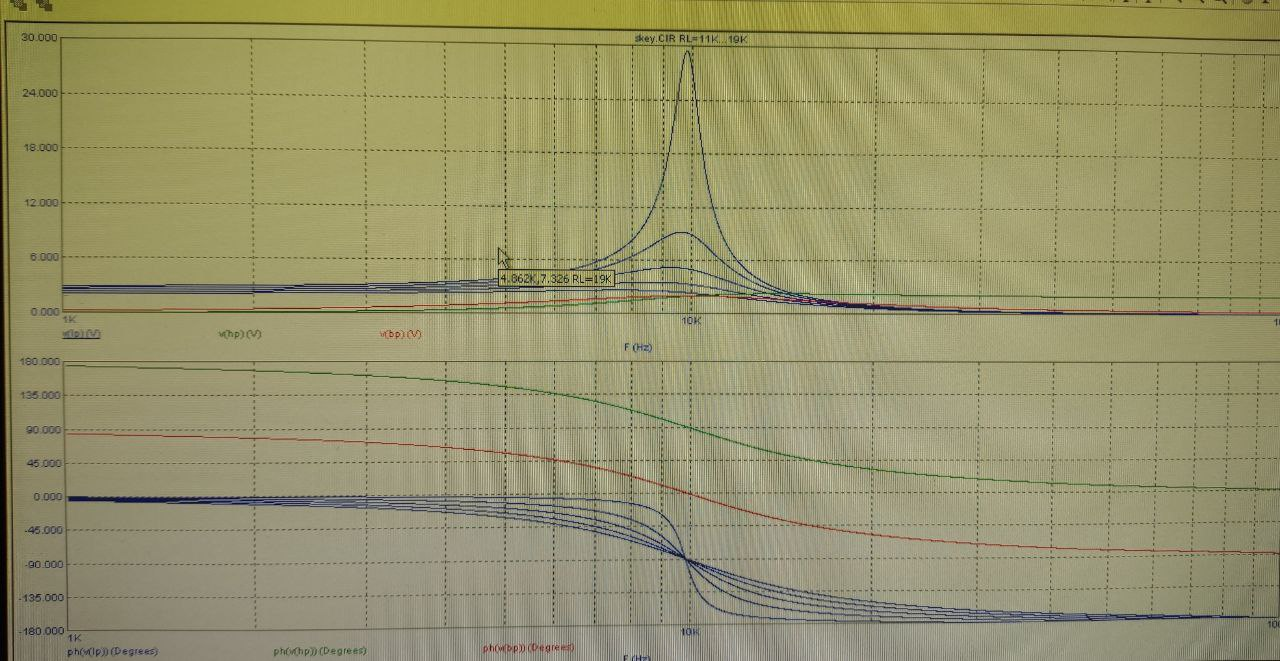
\includegraphics[width=0.9\textwidth]{gr2.jpg}
	\caption{График с варьированием для ФНЧ}
	\label{fig:boiler}
\end{figure}

.

 Измерим пиковые значения усиления при $R_{L,H,P} = 19k$:

\[\textit{ФНЧ}: \quad U = 29,4 \: \text{В}\]
\[\textit{ФВЧ}: \quad U = 28,4 \: \text{В}\]
\[\textit{ПФ}: \quad U = 28,8 \: \text{В}\]

\newpage

2) Исследуем переходные характеристики фильтров и их поведение при варьировании $R_L, R_H, R_P = [11k, 19k|2k].$

.
\begin{figure}[!h]
	\centering
	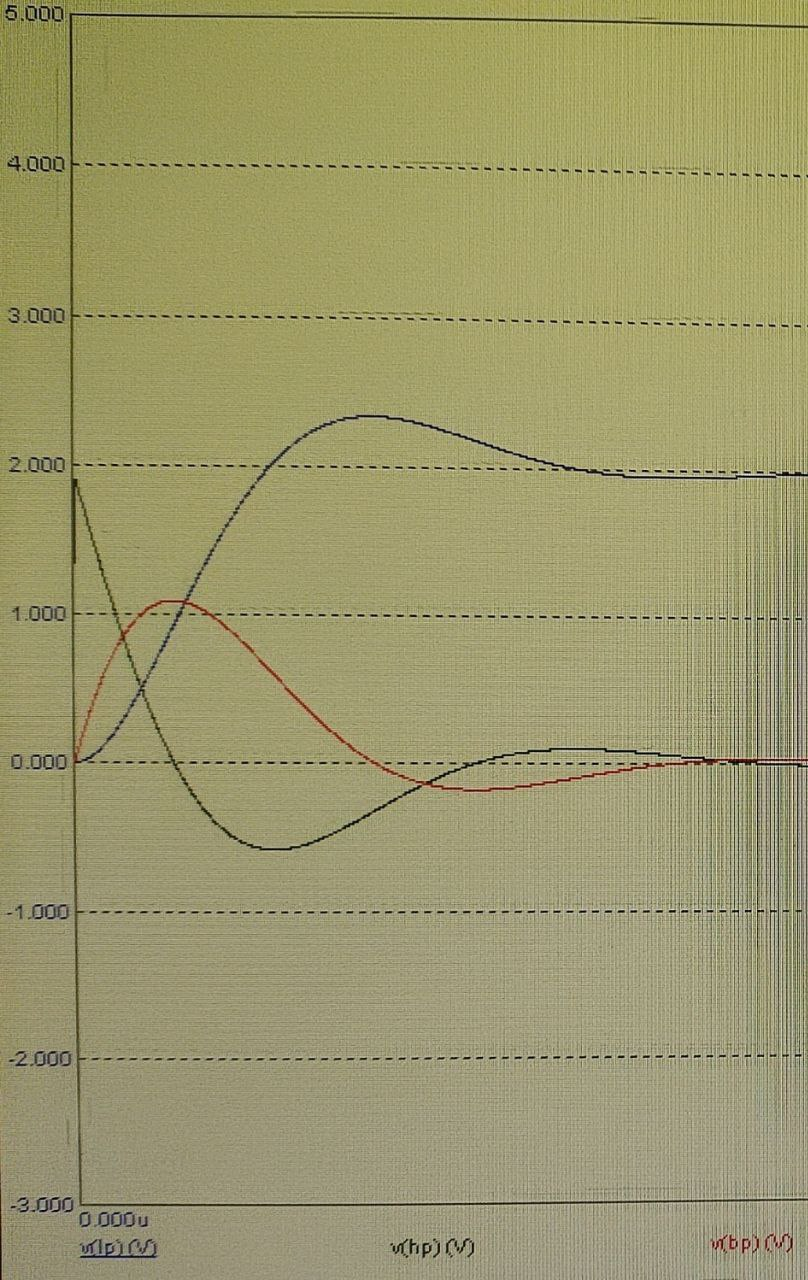
\includegraphics[width=0.5\textwidth]{gr1.jpg}
	\label{fig:boiler}
\end{figure}

.

Как видно по графикам:

Для ФНЧ: $h_\text{ФНЧ} \rightarrow 0 \text{ } (t \rightarrow 0)$, $h_\text{ФНЧ} \rightarrow 2 \text{ } (t \rightarrow \infty)$

Для ФВЧ: $h_\text{ФВЧ} \rightarrow 2 \text{ } (t \rightarrow 0)$, $h_\text{ФВЧ} \rightarrow 0 \text{ } (t \rightarrow \infty)$

Для ПФ: $h_\text{ПФ} \rightarrow 0 \text{ } (t \rightarrow 0)$, $h_\text{ФНЧ} \rightarrow 0 \text{ } (t \rightarrow \infty)$

Что согласуется с теорией и определением этих фильтров.

\newpage

3) Откроем модель $\textit{sk3pole.cir}$ с фильтрами Баттерворта верхних и нижних частот порядка n = 3 на частоту среза $f_0 = 10k$. Проанализируем частотные характеристики фильтров.

.
\begin{figure}[!h]
	\centering
	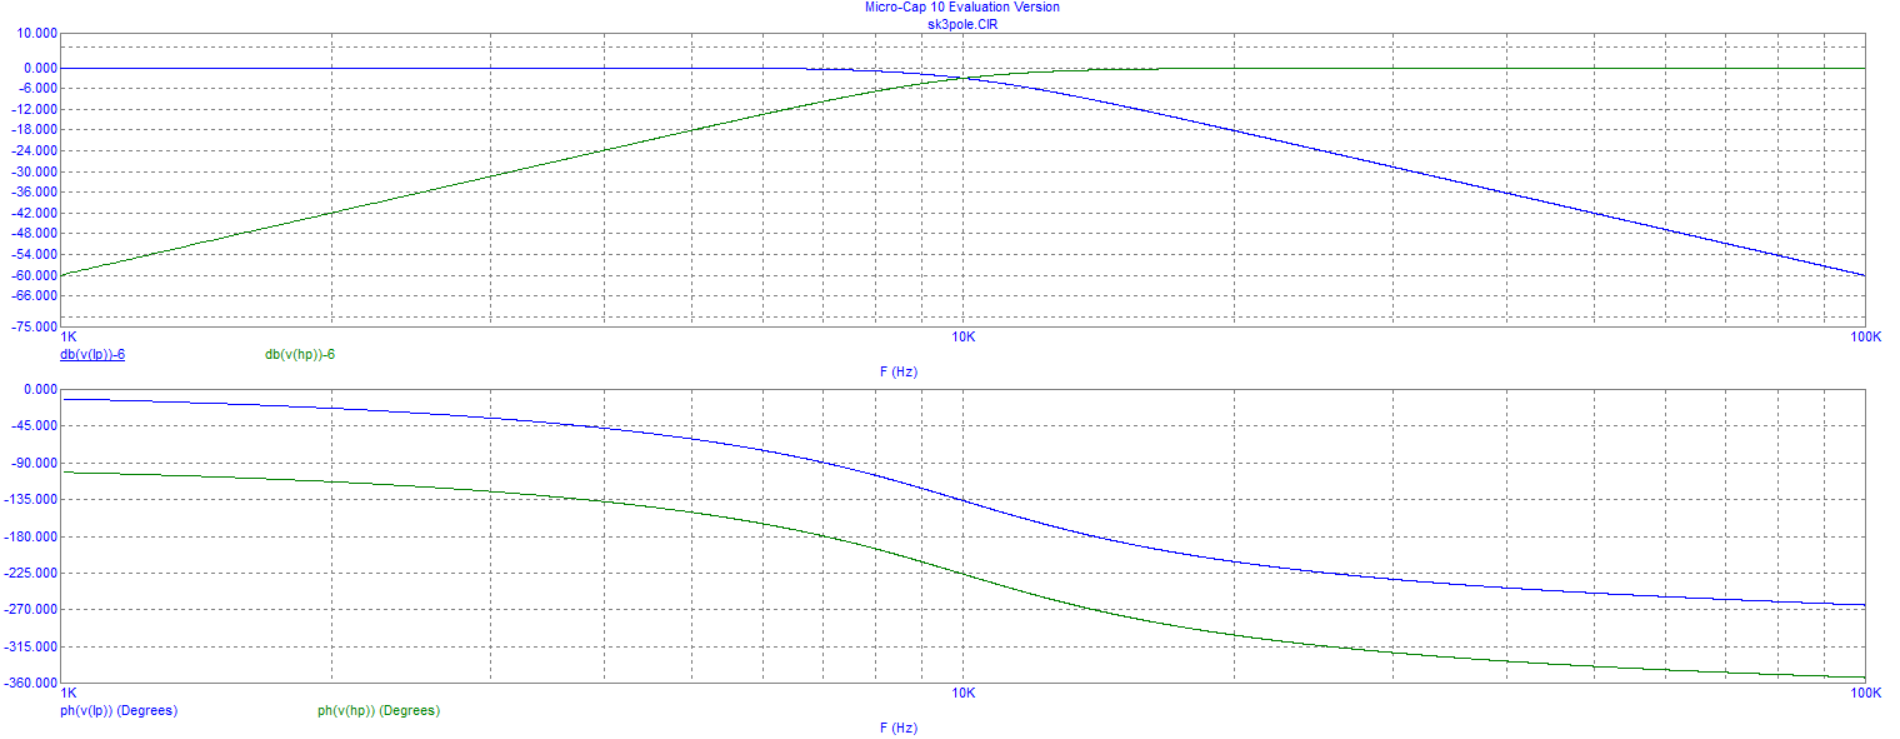
\includegraphics[width=1.0\textwidth]{batt1.png}
	\caption{АЧХ и ФЧХ Баттерворта}
	\label{fig:boiler}
\end{figure}

.

Измерим скорость спада в $dB$ на декаду и затухания на частотах $f_0 / 2, 2f_0$ (на октаву будет в 2 раза больше):

\[\textit{ФВЧ}: \quad f_0 / 2 \rightarrow 57 dB\]
\[\textit{ФВЧ}: \quad 2f_0 \rightarrow 21 dB\]
\[\textit{ФНЧ}: \quad f_0 / 2 \rightarrow -21 dB\]
\[\textit{ФНЧ}: \quad 2f_0 \rightarrow -57 dB\]

Преобразуем их в фильтры Чебышева с $\varepsilon = 1$. Параметры полюсов ФНЧ можно получить в $MatLab$ командой highpass(cheb(3,1)).


\begin{figure}[!h]
	\centering
	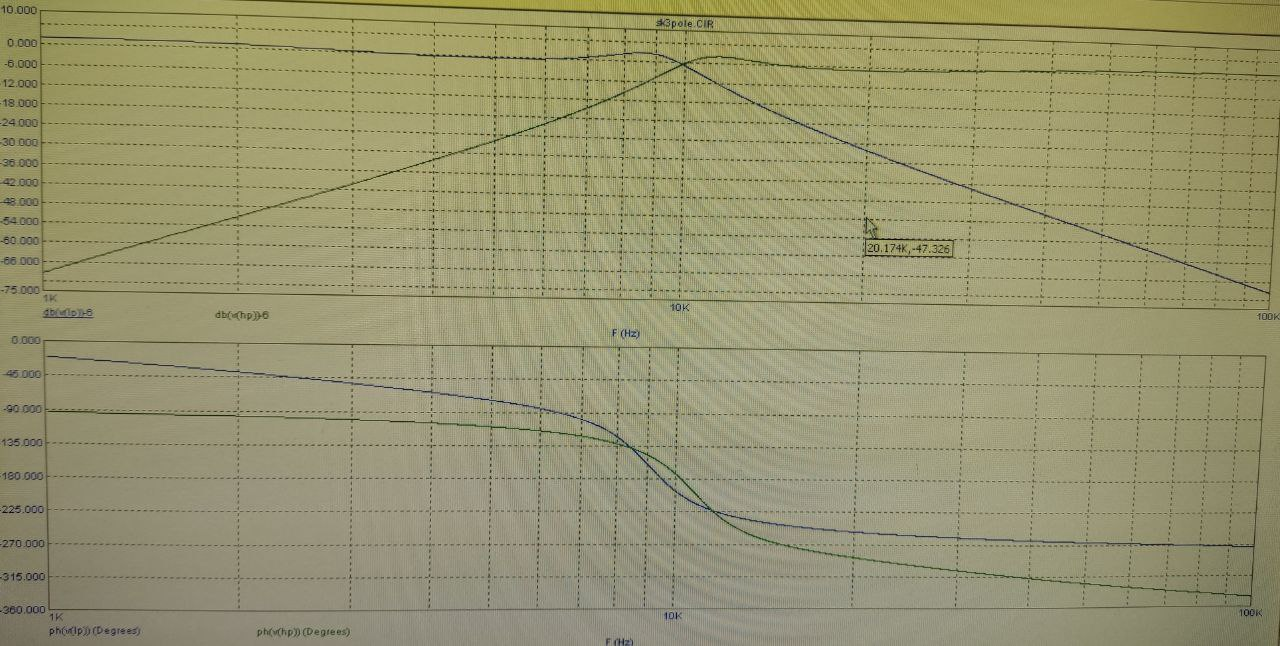
\includegraphics[width=1.0\textwidth]{cheb1.jpg}
	\caption{АЧХ и ФЧХ Чебышева}
	\label{fig:boiler}
\end{figure}


Измерим уровни затухания на частотах $f_0 / 2, 2f_0$ и $f_0 / 10, 10f_0$:

\[\textit{ФВЧ}: \quad f_0 / 2 \rightarrow 68.8 dB\]
\[\textit{ФВЧ}: \quad 2f_0 \rightarrow 0.373 dB\]
\[\textit{ФНЧ}: \quad f_0 / 2 \rightarrow -0.373 dB\]
\[\textit{ФНЧ}: \quad 2f_0 \rightarrow -68.8 dB\]

\newpage

4) Открыв прототип \textit{sk4pole.cir} реализуем 4-полюсной полосовой фильтр Чебышева с $f_0 = 10k, \varepsilon = 1, Q = \frac{f_0}{\bigtriangleup f} = 6$.

\begin{figure}[!h]
	\centering
	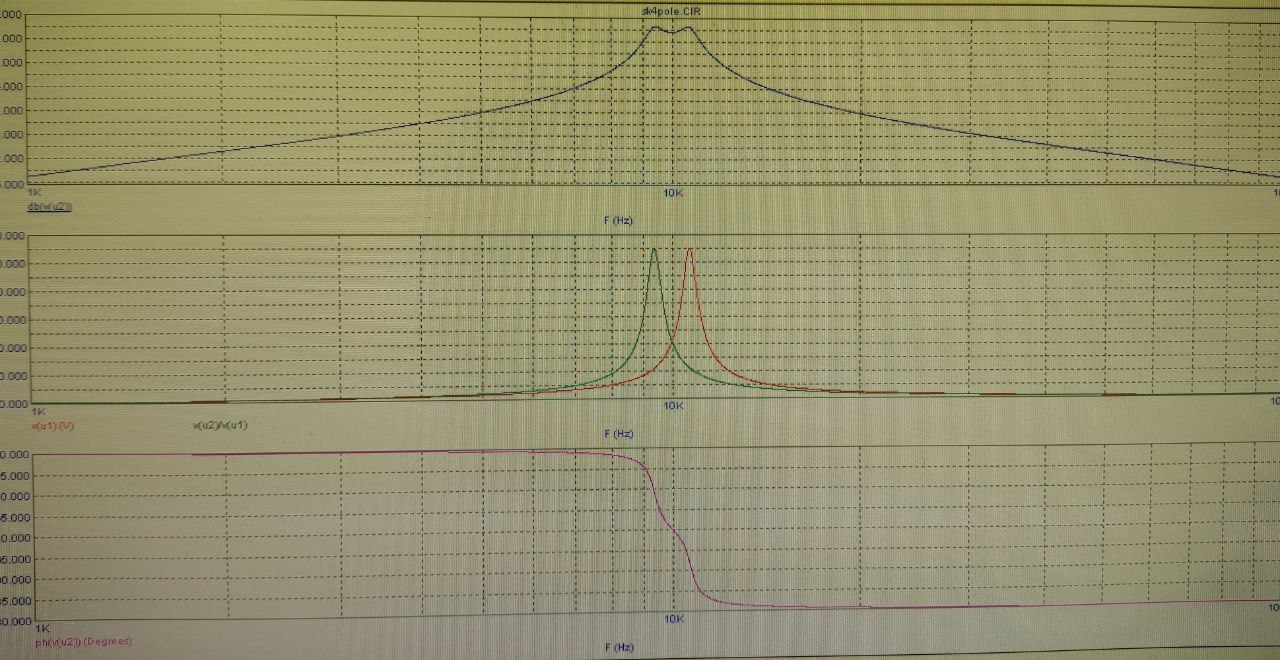
\includegraphics[width=1.0\textwidth]{cheb2.jpg}
	\caption{АЧХ и ФЧХ Чебышева ПФ}
	\label{fig:boiler}
\end{figure}

 Измерим уровни затухания на частотах $f_0 / 2, 2f_0$ и $F_0 / 10, 10f_0$:

\[\textit{ПФ}: \quad 2f_0 \rightarrow -67 dB, \: 10f_0 \rightarrow -40.9 dB\]
\[\textit{ПФ}: \quad f_0 / 2 \rightarrow 67 dB, \: f_0 / 10 \rightarrow 41.1 dB\]

\subsubsection{Вывод}

Проведенное моделирование подтверждает полученные теоретические выкладки.

\subsubsection{Послеслово}

Найдем передаточную функцию полосового звена Саллена-Ки на рисунке. Приведем емкостной импеданс к виду
$Z_C=\frac{1}{p C}=\frac{R}{s} ; s=p R C=\frac{p}{\omega_0}$. К тому же, не ограничивая общности, сопротивление $R$ примем за единицу - безразмерная передаточная функция не зависит от того, в каких единицах измеряются сопротивления. Тогда импедансы резисторов окажуто равными 1 или 2, а импеданс емкости - равным $1 / s$.
Выразим потеницал $u$ на выходе через потенциал в узле $v$ :
$$
u=v \frac{2}{2+\frac{1}{s}} K \Rightarrow v=u \frac{2 s+1}{2 K s} .
$$

Запишем условие равенства нулю токов в узле $v$ :
$$
e-v=v s+v \frac{1}{2+\frac{1}{s}}+v-u \quad \Rightarrow \quad e=v \frac{2\left(s^2+3 s+1\right)}{2 s+1}-u .
$$

Исключив здесь $v$, получим результат.
Формулы для передаточных функций двух других звеньев находятея по аналогии.

\newpage

\subsection{Звенья с двойной обратной связью}

\begin{figure}[!h]
	\centering
	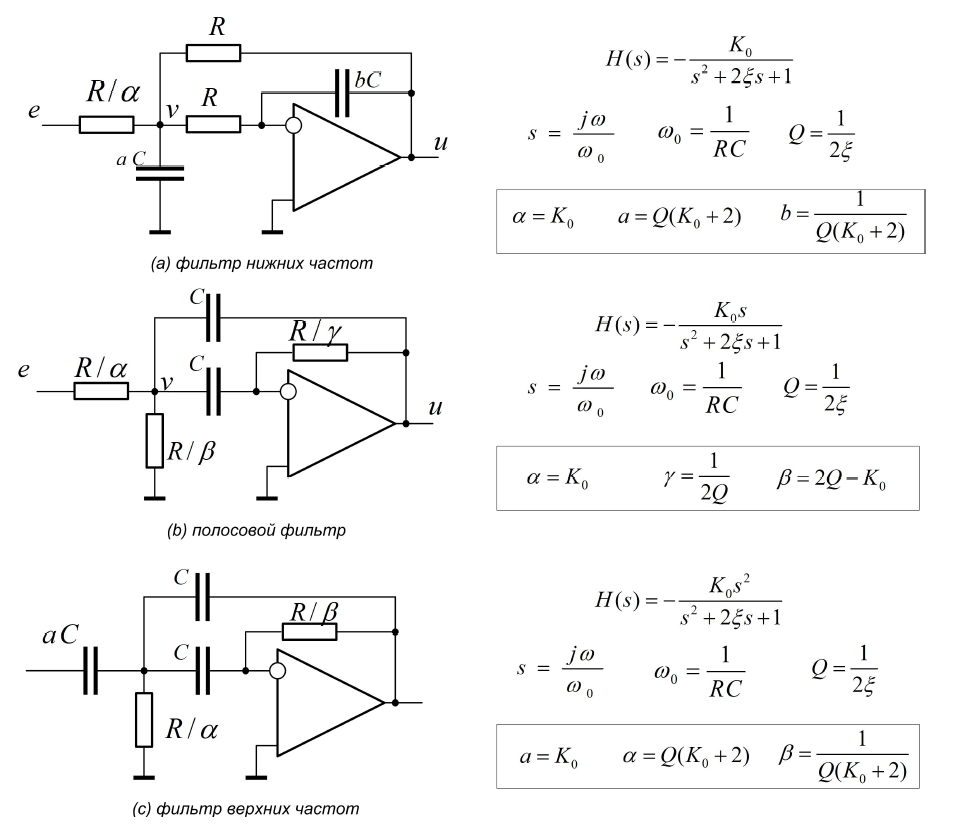
\includegraphics[width=0.9\textwidth]{th2.png}
	\label{fig:boiler}
\end{figure}

\subsubsection{Теория}

Схемы звеньев второго порядка на операционном усилителе, охваченном двойной отрицательной обратной связью, показаны на рис. 2. Все они похожи топологически и различаются только расстановкой резисторов-конденсаторов. Расчет звеньев несколько усложняет схемная избыточность: звено второго порядка характеризуется всего тремя параметрами (резонансная частота $\omega_0$, коэффициент передачи $K_0$ и добротность $Q$ ), а в схеме присутствует целых пять свободных $\mathrm{RC}$-компонентов. В показанных на рисунках схемах свобода выбора несколько ограничена тем, что два из пяти компонентов искусственно объявлены одинаковыми. И все равно задание трех параметров звена не позволяет выбрать оставшиеся четыре компонента однозначно. Приведенные на рисунках расчетные формулы относятся к одному из возможных вариангов выбора, выделенному простотой расчета.

Расчет звена начинается с выбора пары $R, C$, дающей заданную частоту $\omega_0=1 / R C$. Конкретные значения $R$ и $C$ в определенной мере произвольны. Далее подключаются приведенны на рисунке в рамках расчетные формулы, которые позволяют однозначно определить номиналы всех пяти компонентов по заданным параметрам $K_0$ и $Q$.
Звенья с двойной обратной связью всегда устойчивы. Достижимые значения добротности лимитируются в них отношением номиналов компонентов: в любой схеме присутстует компонент со значением, пропорциональным $Q$, и компонент со значением, пропорциональным $1 / Q$. Отношение номиналов этих компонентов растет как $Q^2$, что создает сложности при больших $Q$.

\subsubsection{Выполнение}

1) Откроем прототип \textit{amp1bp.cir} и реализуем полосовое звено с $f_0 = 5k, K_0 = 5, Q = 15$. Измерим ширину полосы по уровню 0.7 = -3dB и пиковое усиление $QK_0$, оценим добротность:

\[\bigtriangleup f = 0.35k\]
\[Q \simeq 14.3\]
\[QK_0 \simeq 75\]

Изучить поведение АЧХ при варьировании $R_2 = [100, 1.3k|200]$. Построить график зависимости частоты пика от $R_2$.

\begin{center}
\begin{tabular}{|c|c|c|c|c|c|c|c|}
\hline 
$f, \: \text{кГц}$ & 4,11 & 4,38 & 4,74 & 5,27 & 6,18 & 7,65 & 12,7 \\ 
\hline 
$R, \: \text{кОм}$ & 1,3 & 1,1 & 0,9 & 0,7 & 0,5 & 0,3 & 0,1 \\ 
\hline 
\end{tabular} 
\end{center}

Построим график

\begin{figure}[!h]
	\centering
	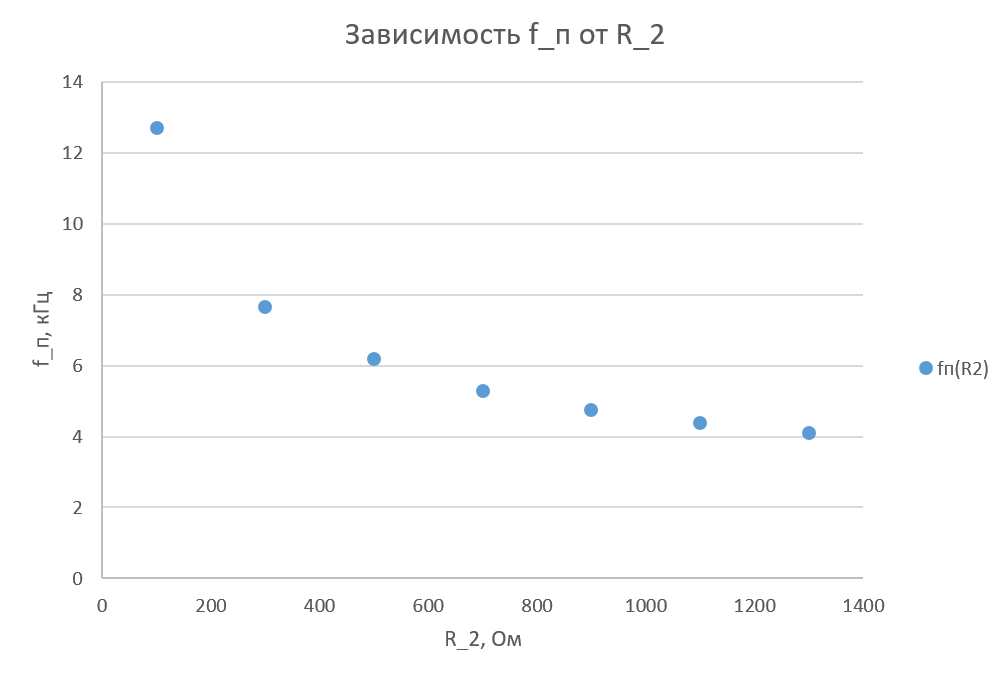
\includegraphics[width=0.9\textwidth]{ex.png}
	\label{fig:boiler}
\end{figure}

\newpage

2) Соберем звено на макетной плате. Экспериментально измерим параметры $K_0, f_0, Q$:

\[f_0 = 4.59 \: \text{кГц}\]

\[K_m = 50\]

\[\bigtriangleup f = 470 \text{ Гц}\]

\[Q \simeq 9.7\]

\[K_0 \simeq 5\]

Как видим, значения сходятся с используемыми теоретическими параметрами.

.

\begin{figure}[!h]
	\centering
	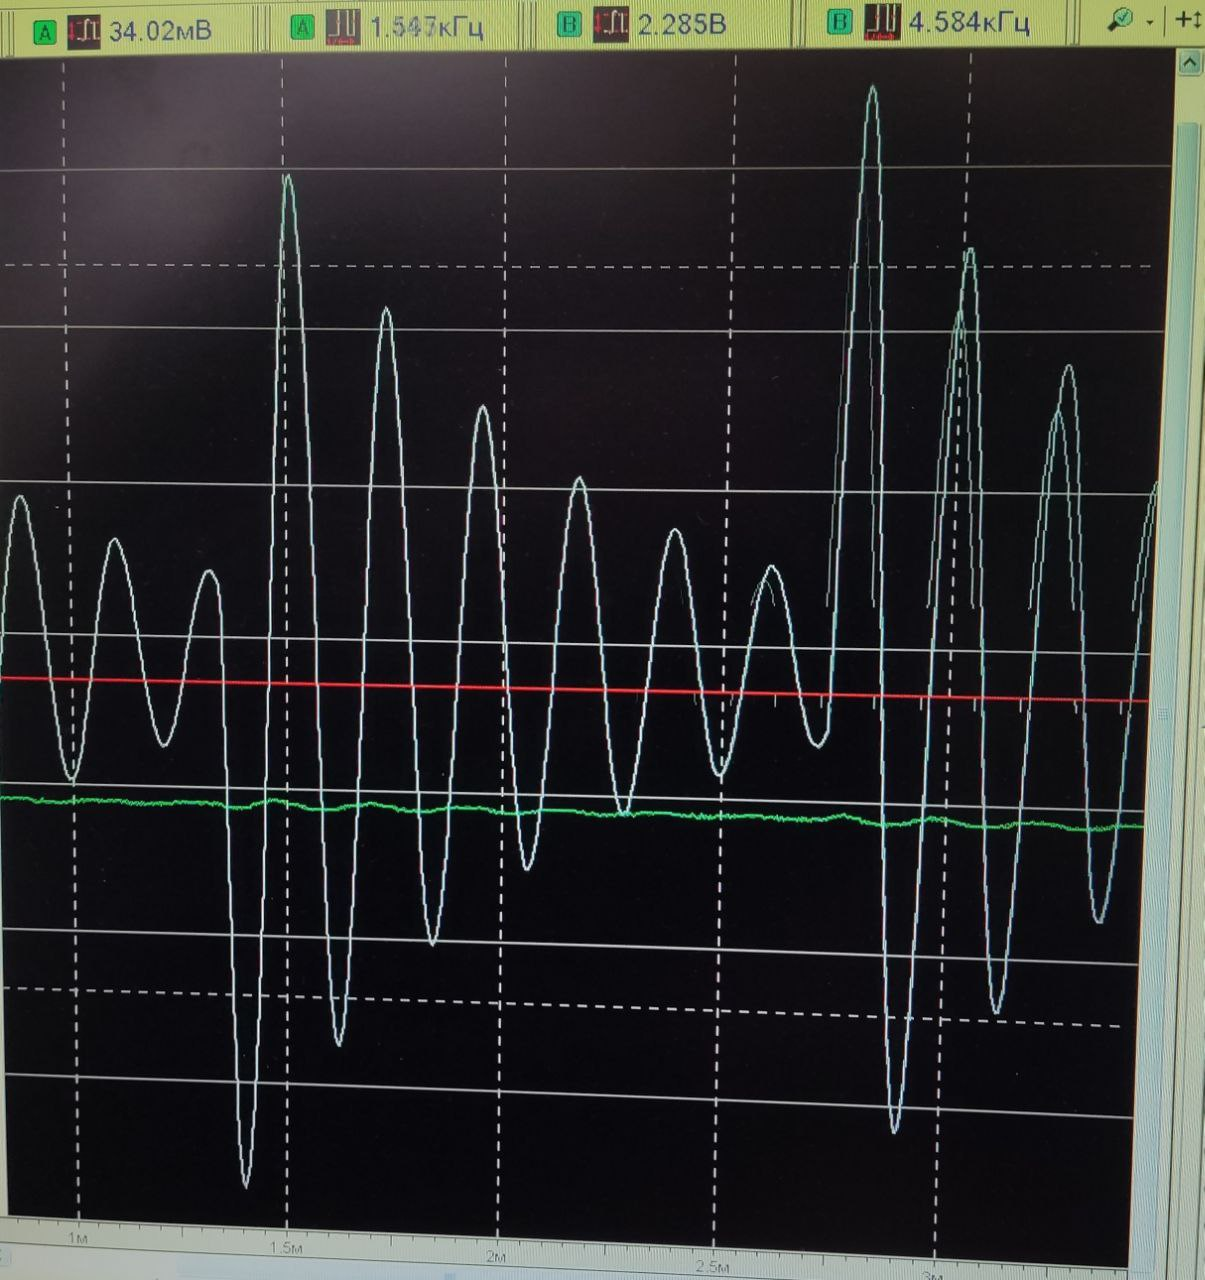
\includegraphics[width=0.7\textwidth]{ht.jpg}
	\label{fig:boiler}
	\caption{h(t) полосового звена при подаче прямоугольного низкочастотного сигнала}
\end{figure}

.

Можем заметить совпадение переходных характеристик собранной и смоделированной схемы.


3) Откроем прототип \textit{cheb6pole.cir} и реализуем шестиполюсный полосовой фильтр Чебышева с параметрами $f_0 = 1k, \varepsilon = 1, Q = 3$.

\begin{figure}[!h]
	\centering
	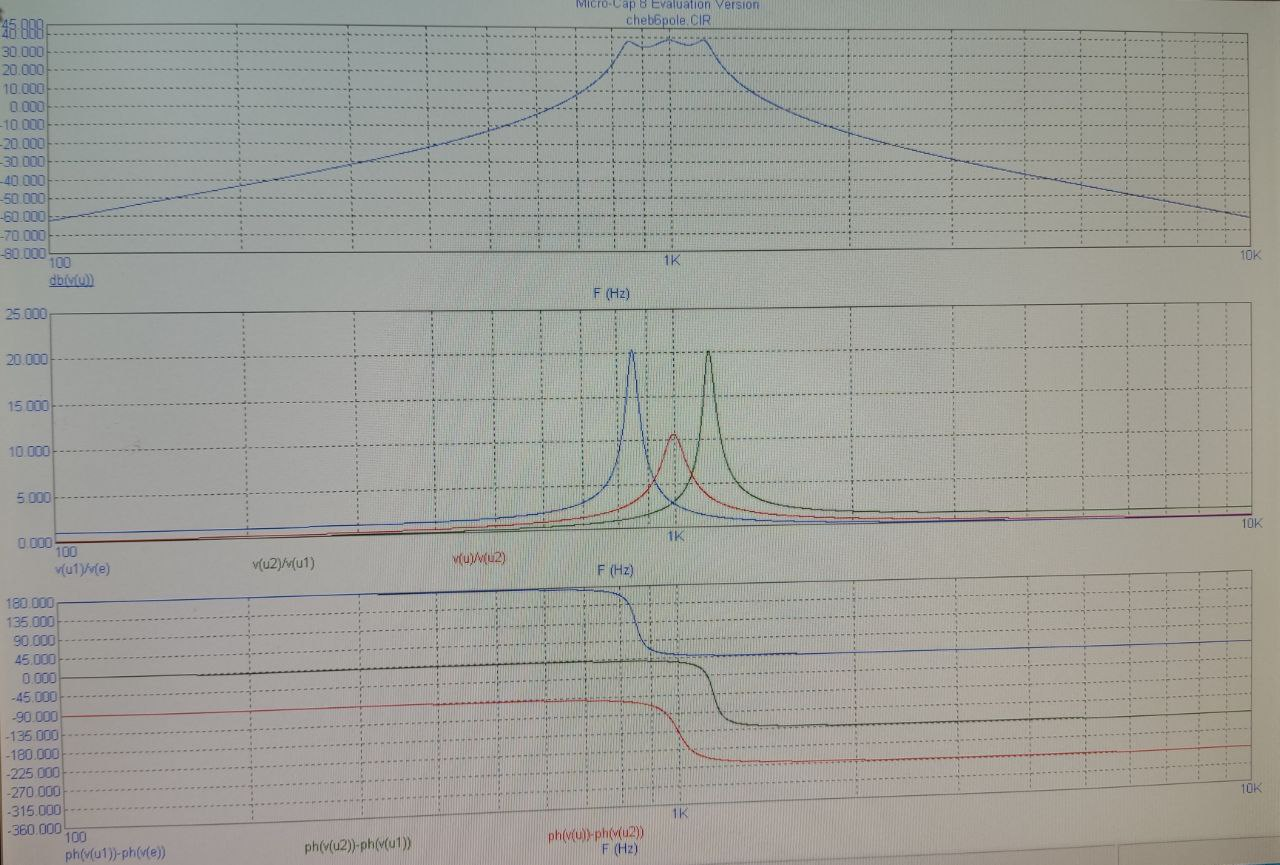
\includegraphics[width=0.9\textwidth]{gr3.jpg}
	\label{fig:boiler}
\end{figure}

Измерим затухания на частотах $0.1k, 0.5k,  2k, 10k$:

\[f = 100: \: 61.7 dB\]
\[f = 500: \: 106.5 dB\]
\[f = 2k: \: 101.1 dB\]
\[f = 10k: \: 61.3 dB\]

\subsubsection{Вывод}

Теория умная, практика умелая, в сумме - красивая лаба.

\section{Вывод}

Результаты моделирования, как и ожидается, тождественны теории, в то время как замеры на макетной плате незначительно от нее отличаются. Все это позволяет сказать, что использованные методы расчета и анализа безинерционных линейных цепей дают хорошие результаты в области применимости.


\end{problem}
\end{document}